%%%%%%%%%%%%%%%%%%%%%%%%%%%%%%%%%%%%%%%%%
% Programming/Coding Assignment
% LaTeX Template
%
% This template has been downloaded from:
% http://www.latextemplates.com
%
% Original author:
% Ted Pavlic (http://www.tedpavlic.com)
%
% Note:
% The \lipsum[#] commands throughout this template generate dummy text
% to fill the template out. These commands should all be removed when 
% writing assignment content.
%
% This template uses a Perl script as an example snippet of code, most other
% languages are also usable. Configure them in the "CODE INCLUSION 
% CONFIGURATION" section.
%
%%%%%%%%%%%%%%%%%%%%%%%%%%%%%%%%%%%%%%%%%

%----------------------------------------------------------------------------------------
%	PACKAGES AND OTHER DOCUMENT CONFIGURATIONS
%----------------------------------------------------------------------------------------

\documentclass{article}
\usepackage{fancyhdr} % Required for custom headers
\usepackage{lastpage} % Required to determine the last page for the footer
\usepackage{extramarks} % Required for headers and footers
\usepackage[usenames,dvipsnames]{color} % Required for custom colors
\usepackage{graphicx} % Required to insert images
\usepackage{caption}
\usepackage{listings} % Required for insertion of code
\usepackage{courier} % Required for the courier font
\usepackage{lipsum} % Used for inserting dummy 'Lorem ipsum' text into the template
\usepackage[colorlinks=true,linkcolor=black,anchorcolor=black,citecolor=black,menucolor=black,runcolor=black,urlcolor=black,bookmarks=true]{hyperref}
\usepackage[table,svgnames]{xcolor}
\usepackage{tabularx}
\usepackage{booktabs}
\usepackage{natbib}
\usepackage{pdfpages}
\usepackage[T1]{fontenc}


% Margins
\topmargin=-0.45in
\evensidemargin=0in
\oddsidemargin=0in
\textwidth=6.5in
\textheight=9.0in
\headsep=0.25in

\linespread{1.1} % Line spacing

% Set up the header and footer
\pagestyle{fancy}
\lhead{\hmwkAuthorName} % Top left header
\chead{\hmwkClass\ (\hmwkClassInstructor\ \hmwkClassTime): \hmwkTitle} % Top center head
\rhead{\firstxmark} % Top right header
\lfoot{\lastxmark} % Bottom left footer
\cfoot{} % Bottom center footer
\rfoot{Page\ \thepage\ of\ \protect\pageref{LastPage}} % Bottom right footer
\renewcommand\headrulewidth{0.4pt} % Size of the header rule
\renewcommand\footrulewidth{0.4pt} % Size of the footer rule

\setlength\parindent{0pt} % Removes all indentation from paragraphs

%----------------------------------------------------------------------------------------
%	CODE INCLUSION CONFIGURATION
%----------------------------------------------------------------------------------------

\definecolor{MyDarkGreen}{rgb}{0.0,0.4,0.0} % This is the color used for comments
\lstloadlanguages{Perl} % Load Perl syntax for listings, for a list of other languages supported see: ftp://ftp.tex.ac.uk/tex-archive/macros/latex/contrib/listings/listings.pdf
\lstset{language=Perl, % Use Perl in this example
        frame=single, % Single frame around code
        basicstyle=\small\ttfamily, % Use small true type font
        keywordstyle=[1]\color{Blue}\bf, % Perl functions bold and blue
        keywordstyle=[2]\color{Purple}, % Perl function arguments purple
        keywordstyle=[3]\color{Blue}\underbar, % Custom functions underlined and blue
        identifierstyle=, % Nothing special about identifiers                                         
        commentstyle=\usefont{T1}{pcr}{m}{sl}\color{MyDarkGreen}\small, % Comments small dark green courier font
        stringstyle=\color{Purple}, % Strings are purple
        showstringspaces=false, % Don't put marks in string spaces
        tabsize=5, % 5 spaces per tab
        %
        % Put standard Perl functions not included in the default language here
        morekeywords={rand},
        %
        % Put Perl function parameters here
        morekeywords=[2]{on, off, interp},
        %
        % Put user defined functions here
        morekeywords=[3]{test},
       	%
        morecomment=[l][\color{Blue}]{...}, % Line continuation (...) like blue comment
        numbers=left, % Line numbers on left
        firstnumber=1, % Line numbers start with line 1
        numberstyle=\tiny\color{Blue}, % Line numbers are blue and small
        stepnumber=5 % Line numbers go in steps of 5
}

% Creates a new command to include a perl script, the first parameter is the filename of the script (without .pl), the second parameter is the caption




%----------------------------------------------------------------------------------------
%	DOCUMENT STRUCTURE COMMANDS
%	Skip this unless you know what you're doing
%----------------------------------------------------------------------------------------

% Header and footer for when a page split occurs within a problem environment
\newcommand{\enterProblemHeader}[1]{
\nobreak\extramarks{#1}{#1 continued on next page\ldots}\nobreak
\nobreak\extramarks{#1 (continued)}{#1 continued on next page\ldots}\nobreak
}

% Header and footer for when a page split occurs between problem environments
\newcommand{\exitProblemHeader}[1]{
\nobreak\extramarks{#1 (continued)}{#1 continued on next page\ldots}\nobreak
\nobreak\extramarks{#1}{}\nobreak
}

\setcounter{secnumdepth}{0} % Removes default section numbers
\newcounter{homeworkProblemCounter} % Creates a counter to keep track of the number of problems

\newcommand{\homeworkProblemName}{}
\newenvironment{homeworkProblem}[1][Problem \arabic{homeworkProblemCounter}]{ % Makes a new environment called homeworkProblem which takes 1 argument (custom name) but the default is "Problem #"
\stepcounter{homeworkProblemCounter} % Increase counter for number of problems
\renewcommand{\homeworkProblemName}{#1} % Assign \homeworkProblemName the name of the problem
\section{\homeworkProblemName} % Make a section in the document with the custom problem count
\enterProblemHeader{\homeworkProblemName} % Header and footer within the environment
}{
\exitProblemHeader{\homeworkProblemName} % Header and footer after the environment
}

\newcommand{\problemAnswer}[1]{ % Defines the problem answer command with the content as the only argument
\noindent\framebox[\columnwidth][c]{\begin{minipage}{0.98\columnwidth}#1\end{minipage}} % Makes the box around the problem answer and puts the content inside
}

\newcommand{\homeworkSectionName}{}
\newenvironment{homeworkSection}[1]{ % New environment for sections within homework problems, takes 1 argument - the name of the section
\renewcommand{\homeworkSectionName}{#1} % Assign \homeworkSectionName to the name of the section from the environment argument
\subsection{\homeworkSectionName} % Make a subsection with the custom name of the subsection
\enterProblemHeader{\homeworkProblemName\ [\homeworkSectionName]} % Header and footer within the environment
}{
\enterProblemHeader{\homeworkProblemName} % Header and footer after the environment
}

%----------------------------------------------------------------------------------------
%	NAME AND CLASS SECTION
%----------------------------------------------------------------------------------------

\newcommand{\hmwkTitle}{A3} % Assignment title
\newcommand{\hmwkDueDate}{Thursday,\ November\ 9,\ 2017} % Due date
\newcommand{\hmwkClass}{\ INTRO. TO INFO RETRIEVAL:\ CS 734} % Course/class
\newcommand{\hmwkClassTime}{} % Class/lecture time
\newcommand{\hmwkClassInstructor}{Dr. Nelson} % Teacher/lecturer
\newcommand{\hmwkAuthorName}{Udochukwu Nweke} % Your name

%----------------------------------------------------------------------------------------
%	TITLE PAGE
%----------------------------------------------------------------------------------------

\title{
\vspace{2in}
\textmd{\textbf{\hmwkClass:\ \hmwkTitle}}\\
\normalsize\vspace{0.1in}\small{Due\ on\ \hmwkDueDate}\\
\vspace{0.1in}\large{\textit{\hmwkClassInstructor\ \hmwkClassTime}}
\vspace{3in}
}

\author{\textbf{\hmwkAuthorName}}
\date{} % Insert date here if you want it to appear below your name

%----------------------------------------------------------------------------------------

\begin{document}

\maketitle

%----------------------------------------------------------------------------------------
%	TABLE OF CONTENTS
%----------------------------------------------------------------------------------------

%\setcounter{tocdepth}{1} % Uncomment this line if you don't want subsections listed in the ToC

\newpage
\tableofcontents
\newpage

%----------------------------------------------------------------------------------------
%	PROBLEM 1
%----------------------------------------------------------------------------------------

% To have just one problem per page, simply put a \clearpage after each problem

\begin{homeworkProblem}


MLN2: using the small wikipedia example, choose 10 words and compute
MIM, EMIM, chi square, dice association measures for full document
\& 5 word windows (cf. pp. 203-205)\\

\textbf{Solution 1:}\\

\lstinputlisting[caption=Association Measure for 10 Words and 5 Word Windows, language=python]{A3.P1.py}

In order to compute term association measures for 10 words from the wiki small corpus I took the following steps: \\
\begin{enumerate}
 \item I read the text files that were downloaded from wiki small corpus from to get HTML text\\
 \item I  used the \textit{boilerplate} removal library (Justext) to extract plain text.\\
 \item I used sklearn \textit{CountVectorizer} to get n-gram vocabulary. This is demonstrated in listing 1, line 271-278.\\
 \item I created a dictionary with key as the term in the collection and value as the files in which the terms occur in (index) 
 \item I used \textit{getAssocMeasuresDocs(a, N, k = 10)} to compute asscionation measures with the formula in Figure 1. For each term, I calculated association measures by referencing the index to find the number of times a term a occurs (Na), the number of times a term b occurs, (Nb), the number of time both terms occur in the index (Nab).
 \item I computed association measures for the five word windows. Some of the examples for the association measures for my chosen word and five word windows are in Table 8-16  the complete file is in \textit{10doc-5wind-words} folder.
\item For five word windows, I processed text and performed the same operations as before but each document was segmented into a group of five word sentences. Some of the examples for my ten chosen word and the top associated terms are in Table 1-8, The complete example file is in \textit{10doc-5wind-words}.
\end{enumerate}






 \begin{table}[h!]
 \centering
 \caption{Top 5 MIM Association for ``Election''}
    \label{tab:first chosen word}
    \begin{tabular}{| l | l| }
     \hline

  Associated Terms &Mutual Information Measure\\
 \hline
 parti&0.008771929824561403\\
 \hline
 patriote& 0.008771929824561403\\
 \hline
 southport& 0.008771929824561403\\
 \hline
 thefa& 0.008771929824561403\\
 \hline
 fabricationfrom& 0.008771929824561403\\
 \hline
 
   \end{tabular}
\end{table}


\begin{table}[h!]
 \centering
 \caption{Top 5 EMIM Association for ``Food''}
    \label{tab:first chosen word}
    \begin{tabular}{ | l | l| }
     \hline

  Associated Terms &Expected Mutual Information\\
 \hline
time & 36.988498354212695\\
 \hline
large & 32.71109290456123\\
 \hline
 water& 31.139744388037478\\
 \hline
 long & 30.34090215895875\\
 \hline
 people & 29.50174435168828\\
 \hline
 
   \end{tabular}
\end{table}


\begin{table}[h!]
 \centering
 \caption{Top 5 Chi-square Association for ``hospital''}
    \label{tab:first chosen word}
    \begin{tabular}{ | l | l| }
     \hline

 Associated Terms &Chi-square\\
 \hline
hospitals & 0.11998634333107323\\
 \hline
health & 0.04862136324886152\\
 \hline
mental & 0.04351811544676538\\
 \hline
medical& 0.04278767992513581\\
 \hline
care & 0.03901883295625831\\
 \hline

 
   \end{tabular}
\end{table}

\begin{table}[h!]
 \centering
 \caption{Top 5 Dice's Association for ``Sports''}
    \label{tab:first chosen word}
    \begin{tabular}{ | l | l| }
     \hline

Associated Terms &Dice’s coefficient\\
 \hline
 sport & 0.13450292397660818\\
 \hline
  football & 0.12334801762114538\\
 \hline
  championship & 0.11940298507462686\\
 \hline
 basketball& 0.11842105263157894\\
 \hline
 stadium & 0.11258278145695365\\
 \hline

 
   \end{tabular}
\end{table}

\begin{table}[h!]
 \centering
    \caption{Top 5 MIM Association for ``Crime'' (5 Word Window)}
    \label{tab:second chosen word}
    \begin{tabular}{ | l | l| }
     \hline

  Associated Terms &Mutual Information Measure\\
 \hline
contentscomparison & 0.009900990099009901\\
 \hline
interpenetration & 0.009900990099009901\\
 \hline
dougbleday & 0.009900990099009901\\
 \hline
bionic & 0.009900990099009901\\
 \hline
 decavalcante & 0.009900990099009901\\
 \hline

   \end{tabular}
\end{table}

\begin{table}[h!]
 \centering
    \caption{Top 5 EMIM Association for ``River'' (5 Word Window)}
    \label{tab:second chosen word}
    \begin{tabular}{ | l | l| }
     \hline

  Associated Terms &Expected Mutual Information Measure\\
 \hline
nelson & 8.012471932229197\\
 \hline
tributary & 7.524054612498825\\
 \hline
wabash & 6.855612505897404\\
 \hline
banks & 6.060661537344706\\
 \hline
 rats & 5.511385944434505\\
 \hline

   \end{tabular}
\end{table}


\begin{table}[h!]
 \centering
    \caption{Top 5 Chi-square Association for ``University'' (5 Word Window)}
    \label{tab:second chosen word}
    \begin{tabular}{ | l | l| }
     \hline

  Associated Terms &Chi-square Measure\\
 \hline
time & 0.006962271180089269\\
 \hline
years & 0.005781562236763527\\
 \hline
new & 0.0056631784106439065\\
 \hline
wikipedia& 0.005068187476213846\\
 \hline
 used & 0.005016678300261902\\
 \hline

   \end{tabular}
\end{table}


\begin{table}[h!]
 \centering
    \caption{Top 5 Dices' Association for ``Book'' (5 Word Window)}
    \label{tab:second chosen word}
    \begin{tabular}{ | l | l| }
     \hline

  Associated Terms &Dices' Measure\\
 \hline
published & 0.030461270670147953\\
 \hline
comic & 0.024759284731774415\\
 \hline
movie & 0.01794616151545364\\
 \hline
lena & 0.015759312320916905\\
 \hline
 wrote & 0.015400410677618069\\
 \hline

   \end{tabular}
\end{table}




\begin{figure}
 \centering
  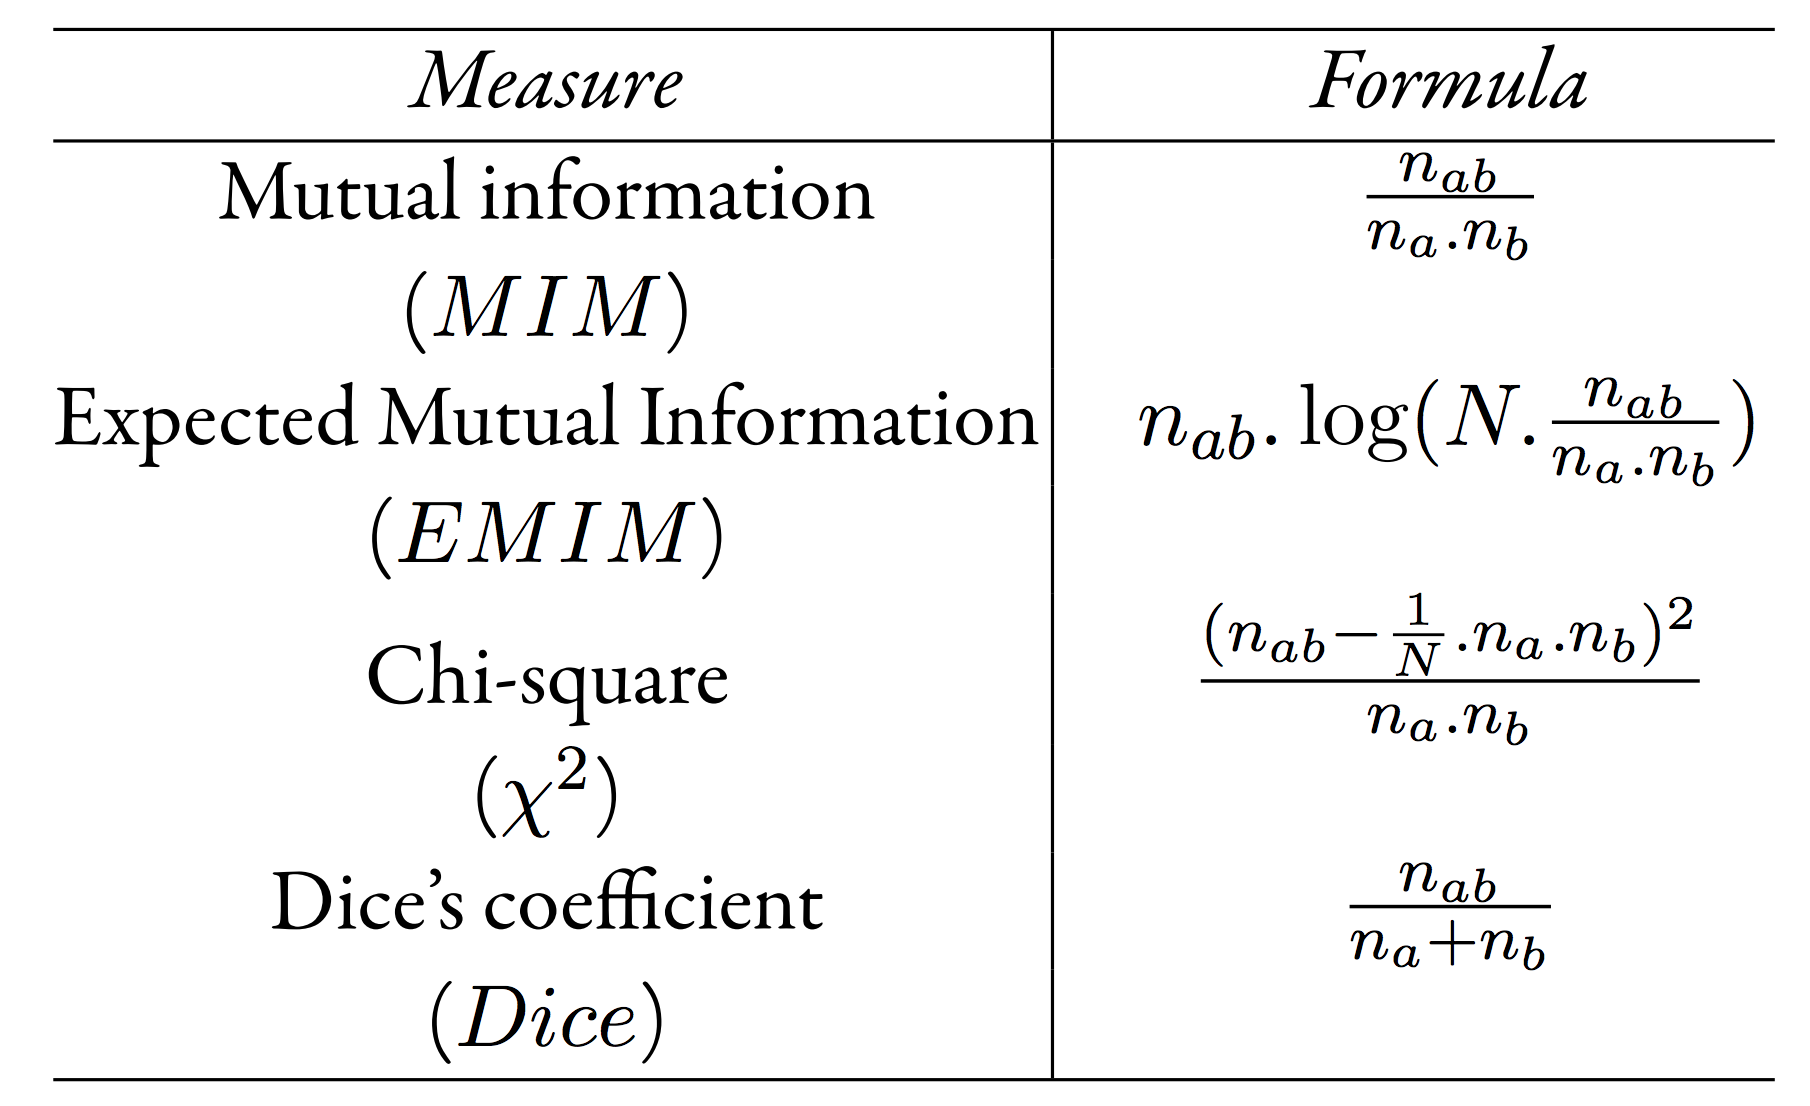
\includegraphics[width=0.5\textwidth]{assocmes.png}
 \caption{Term association measures}
 \end{figure}




 \end{homeworkProblem}
%----------------------------------------------------------------------------------------
% PROBLEM 2
%----------------------------------------------------------------------------------------


\begin{homeworkProblem}

6.1. Using theWikipedia collection provided at the book website, create a sample
of stem clusters by the following process:\\

\begin{enumerate}
\item Index the collection without stemming.
\item Identify the first 1,000 words (in alphabetical order) in the index.
\item Create stem classes by stemming these 1,000 words and recording which
words become the same stem.
\item Compute association measures (Dice’s coefficient) between all pairs of stems
in each stem class. Compute co-occurrence at the document level.
\item Create stem clusters by thresholding the association measure. All terms that
are still connected to each other form the clusters
\end{enumerate}

\textbf{Solution 2:}\\

\lstinputlisting[caption=Extract text from wikismall, language=python]{A3.P3.py}
In order to solve the above problem, I took the following steps: 
\begin{enumerate}
\item I read the text files to get HTML text
\item I  used the \textit{boilerplate} removal library (Justext) to extract plain text.
\item I created a dictionary ( from inverted index), with the key  as the term in the wiki small collection, and the value as the list of files
that include the term. The output is the index called \textit{wiki-small-vocab.json}. 


\item I used \textit{getKAlphabeticalWords(k = 1000)} in Listing 2 to  extract in alphabetical order, 1,000 terms from  \textit{wiki-small-vocab.json} that are words:
That is terms that have only letters of the alphabets: e.g ``gold'' and not ``1gold''. The 
output is \textit{good-1000-words.txt}

\item I used \textit{getStemclasses()} in Listing 2 to create stem classs for the 1,000 words from \textit{good-1000-words.txt} and the words that become the same stem class is in \textit{good-1000-words-stem-classes.txt}.

\item I used \textit{compAssocForPairsInStemClass(stemClasses)} in Listing 2  to compute  association measures (Dice’s coefficient) between all pairs of stems in each stem class and the result is in \textit{good-1000-words-dice.txt}.  The stem classes are represented as a dictionary. The key is the stem, the value is a list of words that map to the stem

\item I used \textit{compAssocForPairsInStemClassThreshold(stemClasses, threshold)} in Listing 2 to create a stem cluster by thresholding the association measure. I used networkx python library to create a graph with nodes as the stems. I added an edge if the Dices' association exceeded the threshold. I used the connected components of the graph to generate the new stem classes. Listing 2, line 115-140

\end{enumerate}
 

\end{homeworkProblem}

%----------------------------------------------------------------------------------------
% PROBLEM 3
%----------------------------------------------------------------------------------------


\begin{homeworkProblem}


6.5. Describe the snippet generation algorithm in Galago. Would this algorithm
work well for pages with little text content? Describe in detail how you would
modify the algorithm to improve it.\\

\textbf{Solution 3:}\\

\lstinputlisting[caption=Extract Galago Snippet Extraction Code, language=python]{P4.py}

The Galago algorithm in Listing 3 can be summarized as follows:
\begin{enumerate}
\item Find a region of text in the document that contains any query term, return a region (left and right) of text based on a predefined text width from the match - \textit{findMatches(), Listing 3 line 6}
\item Combine all regions of text which matched the query term by merging regions that overlap, but break on sentences when predefined merge window size is reached - \textit{combineRegions(), Listing 3, line 6}
\item Highlight terms that match query in regions - \textit{buildHtmlString()}
\end{enumerate}

\textbf{Would this algorithm work well for pages with little text content?}\\

This algorithm set the region for a match to 5 words to the left and 5 words to the right of the position of the query term. Since documents are not typically very small, this threshold is reasonable. The  performance of the algorithm is based on finding region that match the query, not the size of the document. Based on this, the content of the document ought not to affect the performance of the algorithm. The content will only affect the number of candidates to be matched. If the document is too small, there will have lesser candidates to match. The algorithm will work well for pages with lesser content\\ 

\textbf{Ways to improve the Galago algorithm}\\

\begin{enumerate}
\item Exact match should be supplemented with associated words in the same stem class (with high dice or chi-square association), for example, we should match tenses such as: ``fast'' and ``fasting''
\item The algorithm should include regions of alias terms. For example, if the query includes ``Barack,'' we should also generate snippets that match ``Obama''. Also for ``NBA'', we should match regions with ``National Football Association.''
The algorithm should include regions of synonyms terms. For example, if the query include ``Beautiful,'' we should also match regions with ``attractive''
\end{enumerate}





\end{homeworkProblem}

%----------------------------------------------------------------------------------------
% PROBLEM 4
%----------------------------------------------------------------------------------------

\begin{homeworkProblem}

7.7. What is the ``bucket'' analogy for a bigram language model? Give examples.\\

\textbf{Solution 4:}\\

\textbf{Introduction}

A language model is a probability distribution over sequences of words. In other words, a language model assigns probabilities to sequences of words. This shows us how likely a sequence occurs (or generated). Language models are useful in a variety of problems such as spell correction. In Information Retrieval, we use language models to rank each document in a collection by their respective probabilities to a given query. This is called Query likelihood model. This tells us how relevant a document is to a query P(Q|D). In this language model, every document in the collection is a separate language model.\\

\textbf{Bucket analogy}\\

The bucket or bag of words analogy simply means that each document in a collection is represented as a collection of words. There is no order in a bucket. If we represent the document as a collection of single words - we would get a bucket of unigrams, but if we represent the words as a collection of two words - we would get a bucket of bigrams. For example here is a document with the following buckets of unigrams and bigrams:\\

\textbf{Document:} ``The quick brown fox jumped over the lazy dog''\\

\textbf{Unigram bucket:}\\
    The (occurs twice)\\
    quick\\
    brown\\
    fox\\
    jumped\\
    over\\
    lazy\\
    dog\\
    \textbf{Bigram bucket:}\\
    The quck\\
        quick brown\\
        brown fox\\
        fox jumped\\
        jumped  over\\
        over the\\
        the lazy\\
        lazy dog\\

\textbf{Bigram bucket analogy}\\

The bucket analogy for a bigram language model illustrates how we assign probabilities to bigrams with a bigram language model. In other words we measure the probabilities of extracting bigrams from a bucket consisting of bigrams (a document). This means every document is represented as a collection of bigrams. 
The probability of a given term in a query in the bigram language model depends on the probability of the previous term. Generally, the probability of a single word wi is in Figure 2.

\begin{figure}
 \centering
  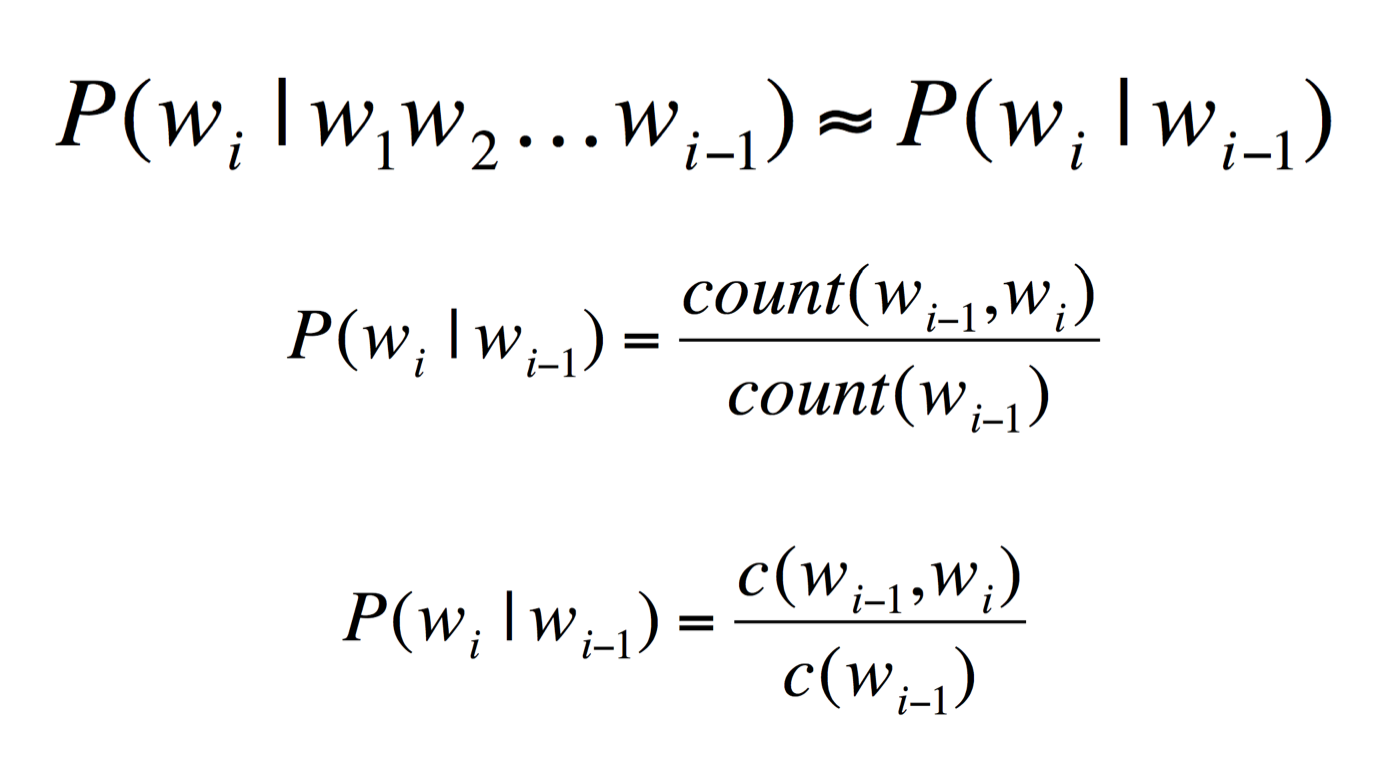
\includegraphics[width=0.5\textwidth]{bigram.png}
 \caption{Measuring n-gram probability}
 \end{figure}

\begin{verbatim}

Document: 
<start>the quick brown fox jumped over</end>
<start>fox jumped over us yesterday</end>
<start>fox jumped over the tent</end>


P(the quick brown) =
P(the | <start>) . P(quick | the) . P(brown | quick) . P(</end> | brown)

P(the | <start>) = 1/3  (1 sentence where “the” after “start”/ 3 sentences with start)
P(quick | the) = 1/2
P(brown | quick) = 1/1

P(the quick brown) = 1/3 . 1/3 . 1 = 0.16666666666



\end{verbatim}






 

\end{homeworkProblem}
%----------------------------------------------------------------------------------------
% PROBLEM 5
%----------------------------------------------------------------------------------------

\begin{homeworkProblem}

MLN1: using the small wikipedia example, choose 10 words and create
stem classes as per the algorithm on pp. 191-192


\textbf{Algorithm}
\begin{enumerate}
\item For all pairs of words in the stem classes, count how often they co-occur in
text windows of W words. W is typically in the range 50-100.
\item Compute a co-occurrence or association metric for each pair. This measures
how strong the association is between the words.
\item Construct a graph where the vertices represent words and the edges are between
words whose co-occurrence metric is above a threshold T.
\item Find the connected components of this graph. These are the new stem classes
\end{enumerate}

\textbf{Solution 5:}\\

\lstinputlisting[caption= Generate stem class based on given algorithm, language=python]{A3.P2.py}
\lstinputlisting[caption= Stem class snippet, language=python]{stemclass.py}
\begin{enumerate}
\item I read the file to get HTML
\item I used \textit{boilerplate} removal (Justext) to get plain text.
\item I applied Porter to plain text to get stem classes. This is achieved with \textit{getStemclasses()} in Listing 4
\item I used \textit{getStemclasses()} in Listing 4 to generate a dictionary with  stem as key, and value as list of terms that map to the stem (stem classes)
\item I used \textit{getAssociationForPair(vocabDict, pair, windowSize)} in Listing 4  to compute  association measures (Dices coefficient) between all pairs of stems in each stem class.  The stem classes are represented as a dictionary. The key is the stem, the value is a list of words that map to the stem
\item I used \textit{optimizeStemClass(oldStemClass, windowSize, threshold))} in Listing 4 to create a stem cluster by thresholding the association measure. I used networkx python library to create a graph with nodes as the stems. I added an edge if the Dice association exceeded the threshold. I used the connected components of the graph to generate the new stem classes with \textit{getStemsClassesSizeKPlus(k=2)} in Listing 4. Snippet of the new stem class is shown in Listing 5 while the complete stem class is saved in \textit{6.1-stem-classes.txt}
\end{enumerate}


\end{homeworkProblem}
%----------------------------------------------------------------------------------------
% PROBLEM 6
%----------------------------------------------------------------------------------------

\begin{homeworkProblem}


7.2. Can you think of another measure of similarity that could be used in the vector space model? Compare your measure with the cosine correlation using some example documents and queries with made-up weights. Browse the IR literature on the Web and see whether your measure has been studied (start with van Rijsbergen’s book).

\textbf{Solution}\\

I came up with a measure of similarity based on multiset - a generalization of sets which allows duplicates. The similarity can be defined as ratio of the size of the multiset intersection and size of the vocabulary. This is very similar to Jaccard, however, Jaccard is meant for sets (no duplicates). My similarity metric generalizes Jaccard because it takes into account the frequency of occurrence of terms.

\textbf{Example1}\\

Doc1: ``Tropical Freshwater Aquarium Fish''\\
Doc2: ``Tropical Fish, Aquarium Care, Tank Setup''\\

Vocabulary vector:
tropical, freshwater, aquarium, fish, care, tank, setup

Doc1 vector: [1, 1, 1, 1, 0, 0, 0]\\
Doc2 vector: [1, 0, 1, 1, 1, 1, 1], \\

Doc1 multiset: {Tropical, Freshwater, Aquarium, Fish}\\
Doc2 multiset: {Tropical, Fish, Aquarium, Care, Tank, Setup}\\

Cosine (Doc1, Doc2) = 0.612372
\begin{verbatim}
Multiset similarity = {Tropical, Freshwater, Aquarium, Fish} intersect {Tropical, 
Fish, Aquarium, Care, Tank, Setup}| / |{tropical, freshwater, aquarium, fish, 
care, tank, setup}|

Multiset similarity = 3/6 = 0.5
\end{verbatim}





\end{homeworkProblem}
%----------------------------------------------------------------------------------------
% PROBLEM 7
%----------------------------------------------------------------------------------------

\begin{homeworkProblem}




6.4. Assuming you had a gazetteer of place names available, sketch out an algorithm for detecting place names or locations in queries. Show examples of the types of queries where your algorithm would succeed and where it would fail.\\

\textbf{Solution}\\

Locations of places are hierarchical in order. For example Old Dominion University is located as follows;\\

Country: USA\\
State: Virginia\\
City: Norfolk\\
Place: Old Dominion University\\

Let my gazetteer be structured hierarchically, for example here is a small portion of the gazetteer:
\begin{verbatim}
Gazetteer:
USA
    Virginia
        Norfolk
            Hampton
            Old Dominion University
            Norfolk State University
        Chesapeake
            Hampton
         
         ...Tide Water Community College
    West Virginia
    ...
...
Canada
\end{verbatim}

\lstinputlisting[caption= Algorithm to identify locations in query, language=python]{identifyLocation.py}
 

\textbf{Positive examples:}\\

Query1: ``Where is Virginia located?''\\
Result: ``Where is [Virginia, State] located?''\\

Query2: ``Directions for Hampton Norfolk''\\
Result: ``Directions for [Hampton, Place] [Norfolk, City]''

\textbf{Negative examples:}\\

Query1: ``Where is  West Virginia located?''\\
Result: ``Where is West [Virginia, State] located?''\\
Failure: Due to multiple words in state name, the tokenizer algorithm only considers single word locations which is not very practical.\\

Query1: ``Where is  Hampton Inn located?''\\
Result: ``Where is [Hampton, Place] Inn located?''\\
Failure: Due to ambiguity in the query\\

As we can see this algorithm is very simplistic and suffers from multiple problems including failure in recognizing aliases of locations. Also it is computationally very expensive to go through the entire gazetteer for each token.



\end{homeworkProblem}
%----------------------------------------------------------------------------------------
% PROBLEM 8
%----------------------------------------------------------------------------------------

\begin{homeworkProblem}


6.9. Give five examples of web page translation that you think is poor. Why do
you think the translation failed?\\

\textbf{Solution}\\
Five example of poor web page translations are: 
\begin{enumerate}
    \item {http://www.cnn.com/2014/01/15/politics/obamacare-spanish-language-site/index.html}
    \item {http://english.cntv.cn/program/learnchinese/specialchinese/index.shtml}
\end{enumerate}
\end{homeworkProblem}

\nocite{*}
\bibliographystyle{plain}
\bibliography{A3Ref}

\end{document}
